\documentclass[11pt]{article}

\usepackage{amsmath,amsthm,amsfonts,amssymb,amsxtra}
\usepackage{pgf,tikz}
\usepackage{mathrsfs}

\renewcommand{\theenumi}{(\alph{enumi})} 
\renewcommand{\labelenumi}{\theenumi}

\pagestyle{empty}
\setlength{\textwidth}{7in}
\setlength{\oddsidemargin}{-0.5in}
\setlength{\topmargin}{-1.0in}
\setlength{\textheight}{9.5in}

\theoremstyle{definition}
\newtheorem{problem}{Problem}

\begin{document}

\noindent{\large\bf MATH 300}\hfill{\large\bf Test \#1}\hfill{\large\bf Fall 2018}\hfill{\large\bf Page 1/6}\hrule

\bigskip
\begin{center}
  \begin{tabular}{|ll|}
    \hline & \cr
    {\bf Name: } & \makebox[12cm]{\hrulefill}\cr & \cr
    {\bf VIP ID:} & \makebox[12cm]{\hrulefill}\cr & \cr
    \hline
  \end{tabular}
\end{center}
\begin{itemize}
\item Write your name and VIP ID in the space provided above.
\item The test has six (6) pages, including this one.
\item Credit for each problem is given at the right of each problem number.
\item Show sufficient work to justify all answers unless otherwise stated in the problem.  Correct answers with
  inconsistent work may not be given credit.
\item No books, notes or calculators are allowed.
\end{itemize}
\hrule

\begin{center}
  \begin{tabular}{|c|c|c|}
    \hline
    &&\cr
       {\large\bf Page} & {\large\bf Max}  & {\large\bf Points} \cr
    &&\cr
       \hline
    &&\cr
       {\Large 2} & \Large 20 &  \cr
    &&\cr
       \hline
    &&\cr
       {\Large 3} & \Large 20 & \cr
    &&\cr
       \hline
    &&\cr
       {\Large 4} & \Large 30 & \cr
    &&\cr
       \hline
    &&\cr
       {\Large 5} & \Large 20 & \cr
    &&\cr
     \hline
    &&\cr
       {\Large 6} & \Large 10 & \cr
    &&\cr       
       \hline\hline
    &&\cr
       {\large\bf Total} & \Large 100 & \cr
    &&\cr
       \hline
  \end{tabular}
\end{center}
\newpage

%%%%%%%%%%%%%%%%%%%%%%%%%%%%%%%%%%%%%%%%%%%%%%%%%%%%%%%%%%%%%%%%%%%%% Page 2
\noindent{\large\bf MATH 300}\hfill{\large\bf Test \#1}\hfill{\large\bf Fall 2018}\hfill{\large\bf Page 2/6}\hrule

\bigskip
\begin{problem}[5 pts]
  Write the following set in set-builder notation:
  \begin{equation*}
    \big\{ \dotsc, -\tfrac{3}{2}, -\tfrac{3}{4}, 0, \tfrac{3}{4}, \tfrac{3}{2}, \tfrac{9}{4}, 3, \tfrac{15}{4},
    \tfrac{9}{2}, \dotsc \big\}
  \end{equation*}

  \vspace{2cm}
\end{problem}
\hrule

\begin{problem}[15 pts--5 pts each]
  Write out the following set by listing its elements between braces:
  \begin{enumerate}
  \item $\{ n \in \mathbb{Z} : 2 < n < 5 \} \times \{ n \in \mathbb{Z} : \lvert n \rvert = 5 \}$.
    \vspace{2cm}
  \item $\big\{ X : X \subseteq \{ 3, 2, a \} \text{ and } \lvert X \rvert = 2 \big\}$
    \vspace{2cm}
  \item $\big\{ X \subseteq \mathscr{P}\big( \{ 1,2,3 \} \big) : \lvert X \rvert \leq 1 \big\}$
    \vspace{7cm}
  \end{enumerate}
\end{problem}
\newpage

%%%%%%%%%%%%%%%%%%%%%%%%%%%%%%%%%%%%%%%%%%%%%%%%%%%%%%%%%%%%%%%%%%%%% Page 3
\noindent{\large\bf MATH 300}\hfill{\large\bf Test \#1}\hfill{\large\bf Fall 2018}\hfill{\large\bf Page 3/6}\hrule

\bigskip
\begin{problem}[10 pts]
  Write the expression involving sets $A$, $B$ and $C$ given by the following Venn diagram:
  \begin{center}
    \begin{tikzpicture}
      \draw[fill=gray] (330:1) circle (1.5);
      \draw[fill=white] (210:1) circle (1.5);
      % \draw[fill=white] (210:1) circle (1.5);
      \draw[fill=gray] ([shift=(185:1.5)]90:1) arc (185:295:1.5) -- ([shift=(5.264:1.5)]210:1) arc (5.264:114.73:1.5);      
      \draw (330:1) circle (1.5);
      \draw (90:1) circle (1.5);
      \draw (90:2.75) node{$B$};
      \draw (210:2.75) node{$A$};
      \draw (330:2.75) node{$C$};
    \end{tikzpicture}
  \end{center}

  \vspace{1cm}
\end{problem}
\hrule

\begin{problem}[10 pts--5 pts each]
  Write the following sets either in set-builder notation, or by listing its elements.  Draw both sets in the plane.
  \begin{enumerate}
  \item $\displaystyle{\bigcup_{\alpha \in [0,1]}[\alpha,1] \times [0,2\alpha^3]}$
  \item $\displaystyle{\bigcap_{\alpha \in [0,1]}[\alpha,1] \times [0,2\alpha^3]}$
  \end{enumerate}

  \vspace{8cm}
\end{problem}

\newpage

%%%%%%%%%%%%%%%%%%%%%%%%%%%%%%%%%%%%%%%%%%%%%%%%%%%%%%%%%%%%%%%%%%%%% Page 4
\noindent{\large\bf MATH 300}\hfill{\large\bf Test \#1}\hfill{\large\bf Fall 2018}\hfill{\large\bf Page 4/6}\hrule

\bigskip

\begin{problem}[10 pts--5 pts each]
  Suppose $A = \{4,3,6,7,1,9\}$ and $B= \{5,6,8,4\}$ have universal set $U=\{0,1,2,\dotsc, 10\}$.
  \begin{enumerate}
  \item Find $A \cap B$.
    \vspace{1cm}
  \item Find $(A^\complement \cap B)^\complement$.
    \vspace{1.5cm}
  \end{enumerate}
\end{problem}
\hrule

\begin{problem}[10 pts]
  Translate the following sentence in symbolic logic, negate it, and translate back to English.
  \begin{quote}
    If $x$ is prime, then $\sqrt{x}$ is not a rational number.
  \end{quote}

  \vspace{4cm}
\end{problem}
\hrule

\begin{problem}[10 pts]
  The \emph{Pierce arrow} $\downarrow$ (also known as the \texttt{NOR} operator or \texttt{NOR} gate) is a logical
  operator defined as follows: If $P$ and $Q$ are statements, then $P \downarrow Q$ is true precisely when both $P$ and
  $Q$ are false.  The computer used in the spacecraft that first carried humans to the moon, the Apollo Guidance
  Computer, was constructed entirely using \texttt{NOR} gates with three inputs.  Answer the following questions:
  \begin{enumerate}
  \item Construct a truth table for $P\downarrow Q$.
    \vspace{2cm}
  \item Show that $P \downarrow P$ is logically equivalent to $\lnot P$.
    \vspace{2cm}
  \item Show that $(P \downarrow Q) \downarrow (P \downarrow Q)$ is logically equivalent to $P \lor Q$.
  \end{enumerate}
\end{problem}
\newpage

%%%%%%%%%%%%%%%%%%%%%%%%%%%%%%%%%%%%%%%%%%%%%%%%%%%%%%%%%%%%%%%%%%%%% Page 5
\noindent{\large\bf MATH 300}\hfill{\large\bf Test \#1}\hfill{\large\bf Fall 2018}\hfill{\large\bf Page 5/6}\hrule

\bigskip

\begin{problem}[10 pts--2 pts each]
  Let $U$ be the set of all students in your class.  Let $C(x)$ be the statement ``$x$ has a cat.'' Let $D(x)$ be the
  statement ``$x$ has a dog.'' Let $F(x)$ be the statement ``$x$ has a ferret.''  Express each of the statements below
  in terms of $U$, $C(x)$, $D(x)$, $F(x)$, quantifiers and logical operations.
  \begin{enumerate}
  \item A student in your class has a cat, a dog and a ferret.
    \vspace{1cm}
  \item All students in your class have a cat, a dog or a ferret.
    \vspace{1cm}
  \item Some student in your class has a cat and a ferret, but not a dog.
    \vspace{1cm}
  \item No student in your class has a cat, a dog and a ferret.
    \vspace{1cm}
  \item For each of the three animals (cat, dog, ferret) there is a student in your class who has one of these animals
    as a pet.
    \vspace{1.5cm}
  \end{enumerate}
\end{problem}
\hrule

\begin{problem}[10 pts]
  Write each of the following statements in the form ``If \makebox[1cm]{\hrulefill}, then \makebox[1cm]{\hrulefill}'' in
  English.
  \begin{enumerate}
  \item I will remember to send you the address only if you send me an e-mail.
    \vspace{1cm}
  \item To be a citizen of this country, it is sufficient that you were born in the United States.
    \vspace{1cm}
  \item If you keep your textbook, it will be useful reference in your future courses.
    \vspace{1cm}
  \item The Red Wings will win the Stanley Cup if their goalie plays well.
    \vspace{1cm}
  \item That you get the job implies that you had the best credentials.
    \vspace{1cm}
  \item The beach erodes when there is a storm.
    \vspace{1cm}
  \item It is necessary to have a valid passport to log on to the server.
  \end{enumerate}
\end{problem}
\newpage

%%%%%%%%%%%%%%%%%%%%%%%%%%%%%%%%%%%%%%%%%%%%%%%%%%%%%%%%%%%%%%%%%%%%% Page 6
\noindent{\large\bf MATH 300}\hfill{\large\bf Test \#1}\hfill{\large\bf Fall 2018}\hfill{\large\bf Page 6/6}\hrule

\bigskip

\begin{problem}[10 pts--2 pts each]
  Consider the statement $Q(x)$ about integer numbers $x \in \mathbb{Z}$: ``$x+1 > 2x$.''  Find the truth value of the
  following:
  \begin{enumerate}
  \item $Q(-1) \land Q(0) \land Q(1)$
    \vspace{1cm}
  \item $\exists x, Q(x)$
    \vspace{1cm}
  \item $\forall x, Q(x)$
    \vspace{1cm}
  \item $\exists x, \lnot Q(x)$
    \vspace{1cm}
  \item $\forall x, \lnot Q(x)$
  \end{enumerate}
\end{problem}

\end{document}
